An anomaly propagation chain may have multiple branches and the number of branches can continue to grow during anomaly propagation chain extension.
Therefore, a main challenge in anomaly propagation chain analysis lies in the exponential growth of the number of possible anomaly propagation branches.
In these branches, some anomalous services and service calls may be irrelevant to the reported availability issue.
To tackle the challenge and improve the efficiency of the analysis, we adopt a pruning strategy to eliminate irrelevant anomalous service calls.
The pruning strategy is based on the assumption that two successive edges (service calls) in an anomaly propagation chain have similar change trends of the corresponding quality metrics.
For example, in Figure~\ref{fig:propagation} the QPS of the edge $S_1 \rightarrow S_4$ should have similar change trend with the QPS of the edge $S_4 \rightarrow S_5$, otherwise the edge $S_1 \rightarrow S_4$ can be pruned.
Similarly, the RT of the edge $S_7 \rightarrow S_9$ and the RT of the edge $S_7 \rightarrow S_{10}$ should have similar change trends with the RT of the edge $S_5 \rightarrow S_7$.

%In this paper, \app~prunes based on the pattern similarity of anomaly propagation~\cite{cscs2013monitorRank}, which effectively improves the performance of anomaly detection.

Similar to the correlation estimation in candidate root cause ranking (see Section~\ref{sec:overview}), we use the Pearson correlation coefficient~\cite{perlationcorrelation} to measure the similarity of the change trends of the corresponding quality metrics of two successive service calls.
For each service call, the service call graph records a quality metric value (e.g., RT, EC, QPS) per minute.
To reflect the latest change trends, we only consider the quality metric values in a latest time window (e.g., the last 60 minutes).
The values for a specific quality metric of a service call in the last $n$ minutes thus can be represented by a vector $X$, where $X_i$ ($1 \leq i \leq n$) represents the value of the $i$th minute.
Given two service calls with the quality metric vectors $X$ and $Y$, their correlation coefficient can be calculated as Equation~\ref{eq:pearson}.

The pruning strategy is executed in the anomaly propagation chain extension process in the following way.
Before adding an anomalous node to the current anomaly propagation chain, check the correlation coefficient of the change trends of the corresponding quality metric of the current edge (service call) with the adjacent upstream/downstream edge.
If the correlation coefficient is lower than a threshold (e.g., 0.7), the current edge will be pruned and the current anomalous node will not be added to the current anomaly propagation chain.
For example, for the example shown in Figure~\ref{fig:propagation}, we will check the correlation coefficient of the QPS change trends of the edge $S_1 \rightarrow S_4$ with the edge $S_4 \rightarrow S_5$.
If the correlation coefficient is lower than the threshold, we will not add $S_1$ to the anomaly propagation chain even if it is a QPS anomalous node.
Similarly, we will check the correlation coefficients of the RT change trends of the edge $S_7 \rightarrow S_9$ and $S_7 \rightarrow S_{10}$ with the edge $S_5 \rightarrow S_7$.



%Where n is the number of samples in the time window, which is set to one hour in our system, $X_{i}$, $Y_{i}$ are the sampled data of variables X and Y, $\bar{X} $ Is the average of X, and $\bar{Y}$ is the average of Y.
%If the similarity value is lower then the threshold(e.g., 0.7), the abnormal propagation path will be cut off, as shown in Figure \ref{fig:cut-edge}, That is, no anomaly detection will be performed on the next node of the abnormal propagation chain.
%In this paper, the data on the edge represents the metrics of the invocation relationships between adjacent nodes, which can well reflect the characteristics of abnormal propagation.
%But the pruning method in this paper is not applicable to the propagation path with node layers less than two, because two-layer nodes have only one edge, and correlation calculation cannot be performed.

%\begin{figure}[ht]
%	\centering
%	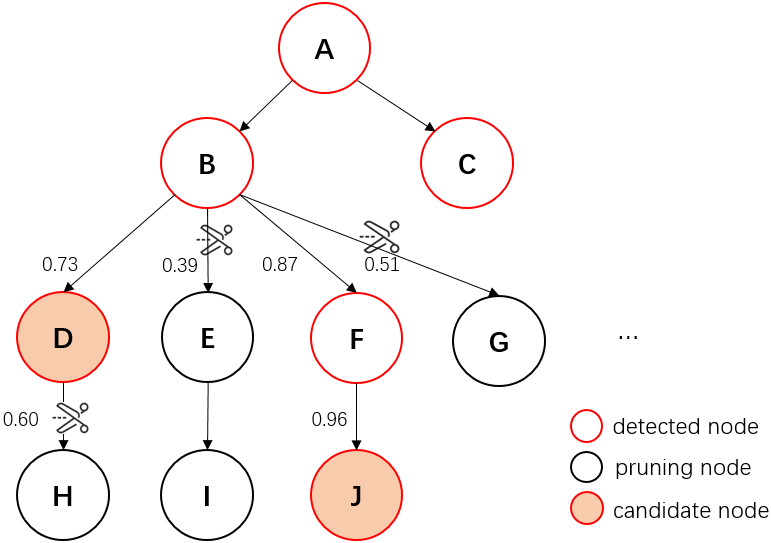
\includegraphics[width=0.42\textwidth]{images/cut-edge.png}
%	\vspace{-8pt}
%	\caption{Pruning on The Graph}\label{fig:cut-edge}
%	\vspace{-10pt}
%\end{figure}
